\documentclass{standalone}
\usepackage{graphicx}	
\usepackage{amssymb, amsmath, amsthm}
\usepackage{color}

\usepackage{tikz}
\usetikzlibrary{math, calc}

\definecolor{light}{RGB}{220, 188, 188}
\definecolor{mid}{RGB}{185, 124, 124}
\definecolor{dark}{RGB}{143, 39, 39}
\definecolor{highlight}{RGB}{180, 31, 180}
\definecolor{gray10}{gray}{0.1}
\definecolor{gray20}{gray}{0.2}
\definecolor{gray30}{gray}{0.3}
\definecolor{gray40}{gray}{0.4}
\definecolor{gray60}{gray}{0.6}
\definecolor{gray70}{gray}{0.7}
\definecolor{gray80}{gray}{0.8}
\definecolor{gray90}{gray}{0.9}
\definecolor{gray95}{gray}{0.95}

\begin{document}

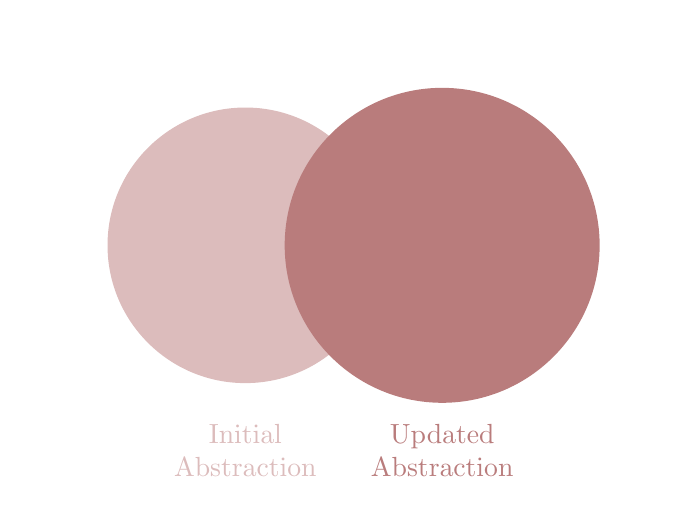
\begin{tikzpicture}[scale=1, thick]
  \draw[white] (-4, -3.25) rectangle (4, 2.75);
  
  \fill[light, dashed] (-1.25, 0) circle (1.75);
  \node[light, align=center] at (-1.25, -2.6) { Initial\\Abstraction };
  
  \fill[mid, dashed] (1.25, 0) circle (2);
  \node[mid, align=center] at (1.25, -2.6) { Updated\\Abstraction };
  
\end{tikzpicture}

\end{document}